\subsection{Long-block TurboAE AWGN check}
The symbolic autoencoder results above use short codewords, so we additionally run a longer-block neural-coding check with a CNN TurboAE-style encoder--decoder at block length \(64\), rate \(1/2\), and AWGN training point \(E_b/N_0=4\,\mathrm{dB}\).
The TurboAE models are trained either through the analytic AWGN channel or through a condition-wise Sinkhorn AWGN surrogate and are then evaluated on the analytic AWGN channel.
This experiment complements the short-block multi-channel SER/BER study.
It checks whether the learned one-shot channel implant remains usable in a longer differentiable coding loop with a different encoder--decoder architecture.

Fig.~\ref{fig:turboae-long-block-curve} shows the resulting BER and BLER curves over \(30\) seeds.
At the \(4\,\mathrm{dB}\) training point, analytic-channel training gives BER \(1.96\times 10^{-3}\) with 95\% CI \(5.21\times 10^{-4}\) and BLER \(8.18\times 10^{-2}\) with 95\% CI \(2.30\times 10^{-2}\).
Training through the condition-wise Sinkhorn surrogate gives BER \(3.30\times 10^{-3}\) with 95\% CI \(4.30\times 10^{-4}\) and BLER \(1.39\times 10^{-1}\) with 95\% CI \(1.91\times 10^{-2}\).
The long-block result therefore preserves the waterfall trend and shows successful surrogate-trained TurboAE optimization, with a measurable gap to analytic-channel training.

\begin{figure}[!b]
\centering
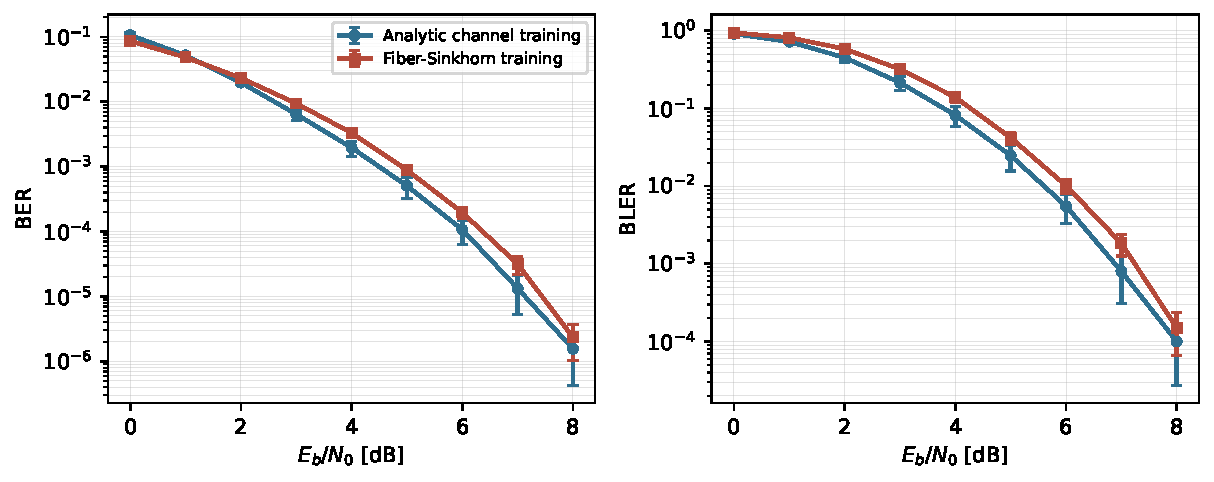
\includegraphics[width=\columnwidth]{figures/turboae_awgn_l64_ber_bler_curve_eval2k.pdf}
\caption{\textbf{Long-block TurboAE AWGN check.} CNN TurboAE models are trained at block length \(64\), rate \(1/2\), and \(E_b/N_0=4\,\mathrm{dB}\), either through the analytic AWGN channel or through the condition-wise Sinkhorn AWGN surrogate. Curves are evaluated on the analytic AWGN channel over \(30\) seeds using \(2000\) evaluation blocks per seed and \(E_b/N_0\) point. The surrogate preserves the qualitative waterfall trend and remains above the analytic-channel training curve.}
\label{fig:turboae-long-block-curve}
\end{figure}
